
\section{Discussion}
\label{sec:discussion}

In this section, we discuss the physical implications of our empirical
findings regarding bow shock shapes.  Our most reliable result is the
average shape of the OB bow shocks from the 227 MIPSGAL sources with
quality rating of 3~stars or higher.  This yields mean values of
\(\Pi = 1.78 \pm 0.06\) and \(\Lambda = 1.72 \pm 0.02\), or median values of
\(\Pi = 1.57\) and \(\Lambda = 1.69\).  The uncertainty quoted on the mean
values is the ``standard error of the mean'':
\(\text{sem} = \sigma / \sqrt{n}\), where \(\sigma\) is the rms dispersion and
\(n\) is the number of sources.  Note that in the case of the
planitude \(\text{sem}(\Pi) = 0.06\) is considerably smaller than
\(\text{mean}(\Pi) - \text{median}(\Pi) = 0.21\), so the latter would be a
more conservative estimate of the uncertainty.\footnote{This is
  because the distribution of \(\Pi\) is approximately log-normal, which
  yields a significant tail towards high values when converted to
  linear space.}  These values can be compared with the predictions of
the thin-shell Wilkinoid model \citep{Wilkin:1996a}, which are
\(\Pi = 1.67\), \(\Lambda = 1.73\) when the bow shock axis lies in the plane
of the sky (following Paper~0, this is defined as the zero point of
the inclination angle, \(i\)).  When the axis is inclined, both
planitude and alatude are predicted to decrease but not by very much,
tending to \(\Pi = 1.5\), \(\Lambda = 1.63\) as
\(\abs{i} \to \ang{90}\) (see \S~5.3 of Paper~0).  The median observed
value\footnote{In the presence of outliers, the median is a more
  robust estimate of the central tendency than is the mean.} falls
squarely inside this range for both the planitude and alatude, which
is a remarkable triumph for the \citet{Wilkin:1996a} model.

On the other hand, turning now to the \emph{variety} of bow shock
shapes, we see that the wilkinoid can no longer explain our results.
The rms dispersions of the planitude and alatude distributions for the
MIPSGAL sources are \(\sigma(\Pi) = 0.87\) and
\(\sigma(\Lambda) = 0.30\) (Tab.~\ref{tab:big-p}), which are respectively 5 times
and 3 times larger than the total range of variation of \(\Pi\) and
\(\Lambda\) predicted for the wilkinoid surface.  Although some of the
dispersion is due to uncertainties in the observations and the fitting
algorithm, this contribution is expected to be small, especially for
the larger, well-resolved sources, for which systematic uncertainties
in the methods for determining \(\Pi\) and \(\Lambda\) will
dominate. Conservative upper limits to the relative size of these
uncertainties were estimated in \S~7 of Paper~0 to be \(< 20\%\) for
\(\Pi\) and \(< 10\%\) for \(\Lambda\), whereas the observed dispersions are
roughly twice as large: \(\sigma(\Pi)/\Pi = 55\%\) and \(\sigma(\Lambda)/\Lambda = 18\%\).


\begin{figure}
  \centering
  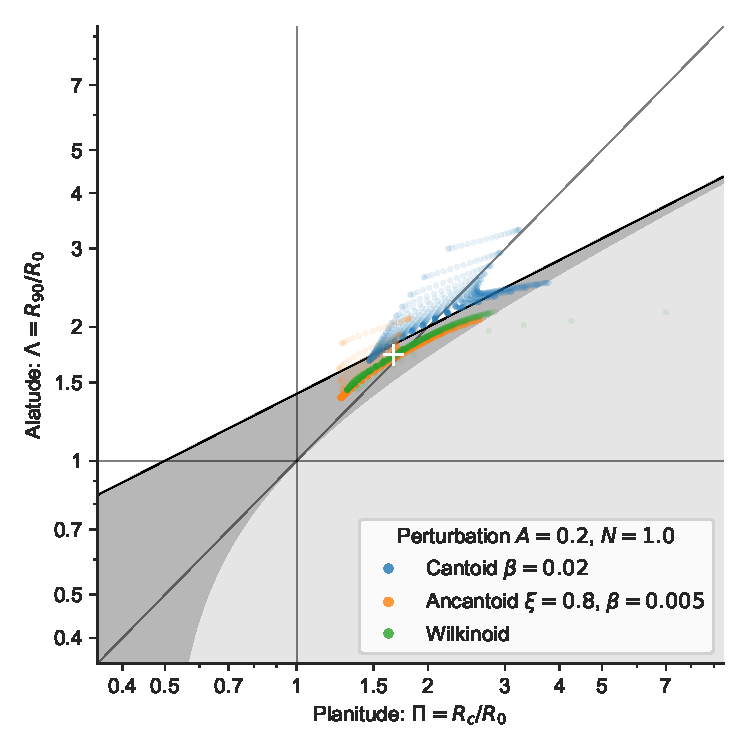
\includegraphics[width=\linewidth]
  {figs/wave-R90-vs-Rc-A020-N10}
  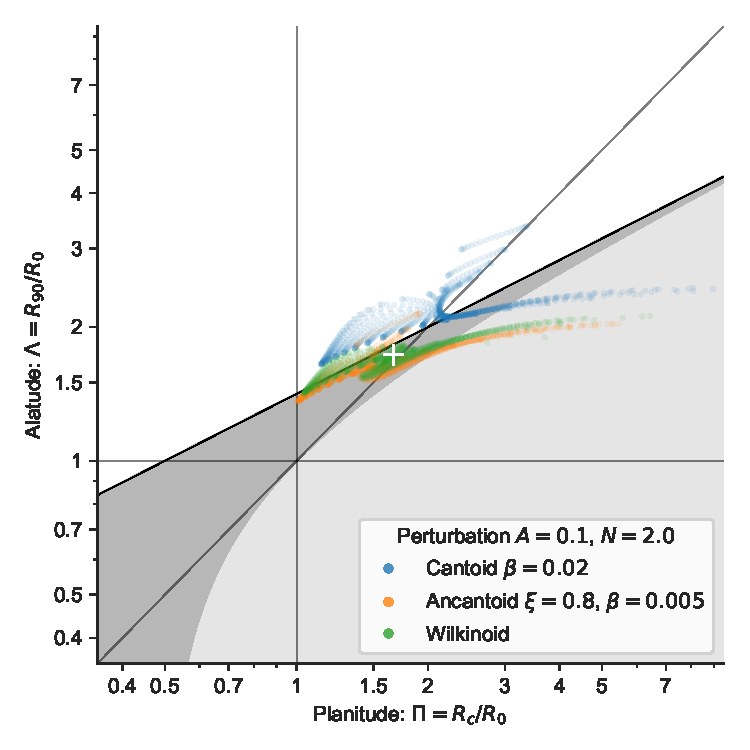
\includegraphics[width=\linewidth]
  {figs/wave-R90-vs-Rc-A010-N20}
  \caption{Diagnostic diagram for perturbed shapes}
  \label{fig:perturb-Rc-R90}
\end{figure}



%%% Local Variables:
%%% mode: latex
%%% TeX-master: "obs-bowshocks"
%%% End:
